\documentclass[11pt]{article}
\usepackage{shared/hanzocover}
\usepackage[utf8]{inputenc}
\usepackage{amsmath,amssymb,amsthm}
\usepackage{graphicx}
\usepackage{booktabs}
\usepackage{hyperref}
\usepackage{xcolor}
\usepackage{listings}
\input{shared/lstlang}
\usepackage{tikz}
\usetikzlibrary{shapes,arrows,positioning,fit}

\definecolor{codegreen}{rgb}{0,0.6,0}
\definecolor{codegray}{rgb}{0.5,0.5,0.5}
\definecolor{codepurple}{rgb}{0.58,0,0.82}
\definecolor{backcolour}{rgb}{0.95,0.95,0.92}

\lstdefinestyle{mystyle}{
    backgroundcolor=\color{backcolour},
    commentstyle=\color{codegreen},
    keywordstyle=\color{codepurple},
    numberstyle=\tiny\color{codegray},
    stringstyle=\color{codegreen},
    basicstyle=\ttfamily\footnotesize,
    breakatwhitespace=false,
    breaklines=true,
    captionpos=b,
    keepspaces=true,
    numbers=left,
    numbersep=5pt,
    showspaces=false,
    showstringspaces=false,
    showtabs=false,
    tabsize=2
}
\lstset{style=mystyle}

\newtheorem{theorem}{Theorem}
\newtheorem{lemma}{Lemma}
\newtheorem{proposition}{Proposition}
\newtheorem{definition}{Definition}

\title{Continuously-Learning Private AI: Self-Improvement and Privacy in the Hanzo Native Stack}
\author{Hanzo Dev \\ \texttt{dev@hanzo.ai} \\ \textit{Hanzo AI}}
\date{June 2026}

\begin{document}

\hanzocoverpage

\begin{abstract}
A private continuously-learning model is three loops bolted together: an \emph{inference} loop that serves a user and captures its own interactions; a \emph{curation} loop that filters, redacts, and de-duplicates that capture into safe training data; and a \emph{training} loop that folds the data back into cheap, swappable per-user and per-task deltas. We design this system on the Hanzo native stack, which already owns the hard inference substrate---a ROCm decode matvec at the memory-bandwidth wall, at effective parity with llama.cpp (an 8B dense transformer at Q8\_0, decode $24.5$ tokens/s, $0.98\times$ the $25.05$ tokens/s of llama.cpp HIP on one gfx1151 / AMD~8060S)---and a real, tested reinforcement-learning trainer (a ported GRPO implementation with passing smoke tests). It does \emph{not} yet own the curation loop (no span-level PII redactor exists) or a Rust federated control plane (it is Python-only in the \texttt{zen/gym} project). We are explicit throughout about which pieces are real, which are ported, and which are research. We then formalize the two privacy-and-stability invariants the design rests on: a \emph{privacy invariant}---no personally-identifiable token enters the training set because a guard filter is applied to every datum before training---which we prove holds under the curation pipeline; and a \emph{bounded-forgetting} guarantee for delta-personalization---a frozen quantized base implies zero base-capability drift, with all change localized to low-rank adapters---which we also prove. We are honest about the two failure modes that can sink the system: model collapse from self-training, and privacy leakage through the delta.
\end{abstract}

\section{Introduction}

The case for keeping a learning loop on the user's own machine is not ideological; it is the only architecture in which raw user data never has to move. That requires both local inference \emph{and} local training to be fast enough to be invisible. This paper argues that the Hanzo native stack is unusually well positioned to host such a loop, designs the complete system, and is scrupulous about the boundary between what is built and what is aspirational.

Throughout, we are precise about the status of every claim, and we make the distinction in the prose rather than in shorthand: we say plainly when code exists today and was read from source, when a capability was ported from a named open-source project, when a piece is genuinely new Hanzo intellectual property, when something is buildable on the existing substrate with bounded engineering but is not yet built, and when a problem is open research. The reader should assume nothing here is built unless the text says so.

\paragraph{Inference is there.}
A sustained optimization campaign~\cite{hanzorocm} drove the 8B model's Q8\_0 decode from $8.5$ to $\mathbf{24.5}$~tokens/s, i.e. $0.98\times$ the llama.cpp HIP figure of $25.05$~tokens/s---effective parity. The mechanism was a rewrite of the unified quantized matvec inner loop from a serial whole-warp-per-block scheme to a \emph{lane-strided, warp-reduce} scheme, taking the dominant feed-forward shapes from roughly $45\%$ to $\mathbf{97\%}$ of the $217$~GB/s memory roofline; the matvec is now bandwidth-wall-bound. Prefill is $1015$~tokens/s, or $0.86\times$ llama.cpp's $1176$~tokens/s---the harder remaining axis, requiring a multi-wave WMMA flash-attention kernel. Mixture-of-experts (MoE) decode improved $2\times$ ($6.34 \to 13.6$~tokens/s) via the same unified core plus a resident-bank cache. These are honest numbers on a single gfx1151 (AMD~8060S / Strix~Halo): decode is at parity, prefill trails, and beating llama.cpp on ROCm would require a PagedAttention keystone that has not yet paid off. The point for \emph{this} paper is narrower: a model that serves the user at $\sim$$25$~tokens/s decode is fast enough to also be the data generator for its own training, and the same quantized weights it serves from are the base on which deltas sit.

\paragraph{Training is partly there.}
As detailed in Section~\ref{sec:substrate}, the autograd engine, the optimizers, the checkpoint seam, and one full reinforcement-learning trainer are real and tested; a generic supervised fine-tuning (SFT) trainer that actually updates weights, and low-rank adapter injection, are not.

\paragraph{Contributions.}
\begin{itemize}
    \item A complete three-loop architecture (serve--capture, curate, train, optionally federate) for on-device private continual learning, mapped onto concrete Hanzo source files with explicit reality tags.
    \item A formal \emph{privacy invariant} (Definition~\ref{def:privinv}) and a proof that the curation pipeline maintains it (Proposition~\ref{prop:privinv}).
    \item A formal \emph{bounded-forgetting} guarantee for delta-personalization over a frozen quantized base (Proposition~\ref{prop:forget}), with proof.
    \item An honest treatment of the two existential failure modes---model collapse and delta leakage---and a prioritized build order separating bounded engineering from genuine research.
\end{itemize}

\section{The Loop}
\label{sec:loop}

The system is three coupled loops that never let raw data leave the device. Figure~\ref{fig:loop} sketches the data path.

\begin{figure}[t]
\centering
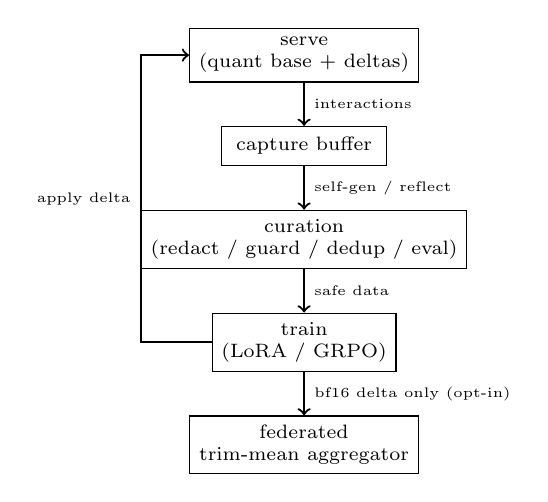
\begin{tikzpicture}[
    node distance=0.55cm,
    box/.style={rectangle, draw, minimum width=2.1cm, minimum height=0.5cm, align=center, font=\scriptsize},
    arrow/.style={->, thick}
]
\node[box] (serve) {serve\\(quant base $+$ deltas)};
\node[box, below=of serve] (capture) {capture buffer};
\node[box, below=of capture] (curate) {curation\\(redact / guard / dedup / eval)};
\node[box, below=of curate] (train) {train\\(LoRA / GRPO)};
\node[box, below=of train] (fed) {federated\\trim-mean aggregator};

\draw[arrow] (serve) -- node[right,font=\tiny]{interactions} (capture);
\draw[arrow] (capture) -- node[right,font=\tiny]{self-gen / reflect} (curate);
\draw[arrow] (curate) -- node[right,font=\tiny]{safe data} (train);
\draw[arrow] (train.west) -- ++(-0.9,0) |- node[left,font=\tiny,pos=0.25]{apply delta} (serve.west);
\draw[arrow] (train) -- node[right,font=\tiny]{bf16 delta only (opt-in)} (fed);
\end{tikzpicture}
\caption{On-device continual-learning loop. Raw data never leaves the device; only an optional bf16 LoRA delta crosses the wire to the cross-device aggregator.}
\label{fig:loop}
\end{figure}

\paragraph{Stage A---serve and capture.}
The quantized base model (e.g. the 8B model at Q8\_0), served through the real $460$-LoC \texttt{engine/hanzo-engine/src/models/quantized\_qwen3.rs} in the tree today, answers the user. Interactions---prompt, response, and any explicit or implicit feedback (thumbs, edits, acceptance of a code completion)---land in a local capture buffer. This buffer is plumbing that is buildable on the existing substrate but not yet built.

\paragraph{Stage B---self-generate / reflect.}
Beyond raw capture, the model manufactures training data: (i)~\emph{self-instruct}-style synthetic prompts in the user's domain; (ii)~\emph{self-critique / reflection}---generate an answer, then generate a critique-and-revise pass, keeping the revised answer as the target (a distillation-from-self signal). The honesty boundary here: the \texttt{zen/gym} reconnaissance confirmed it ships knowledge distillation (logit / top-$k$ and online-teacher), but the reflection / self-critique data-manufacturing described here is open research---a recipe, not ported code.

\paragraph{Stage C---curation.}
The gate that makes the loop private and stable: PII redaction, a safety gate, dedup / diversity, and an eval gate (Sections~\ref{sec:privacy} and~\ref{sec:collapse}). Nothing leaves this stage that contains personal data or that would degrade the model.

\paragraph{Stage D---train.}
Curated samples drive a parameter-efficient update---per-task / per-user LoRA deltas (cheap, swappable; Section~\ref{sec:delta})---via the native trainers (Section~\ref{sec:substrate}). For preference-shaped feedback (the user picked answer~A over~B), a DPO/KTO-style loss; for reward-shaped feedback (a score, a passing test), the real GRPO trainer. The update touches only the delta, never the frozen quantized base, which is what makes it cheap and forgetting-resistant (Section~\ref{sec:delta}).

\paragraph{Stage E---optional federation.}
If the user opts in to contribute, only the bf16 LoRA delta crosses the wire to a trim-mean aggregator (Section~\ref{sec:fed}). Raw data never does. This stage exists today only as a ported design, not in Rust: it is implemented in Python in \texttt{zen/gym} and is absent from the Hanzo \texttt{net/} crate.

\section{Privacy: What the Guard Must Do, and What It Cannot}
\label{sec:privacy}

The privacy property is defense in depth on the data path between capture and training. An early framing described \texttt{zen-guard} as ``the Rust filter family.'' The code says otherwise, and getting this right is load-bearing.

\paragraph{Ground truth on zen-guard.}
Read from the three \texttt{zen-guard} repositories: it is a \emph{model family}---a generative, streaming safety-moderation classifier that emits per-turn safety and PII labels---with \emph{zero Rust}, no \texttt{Cargo.toml}, no \texttt{.rs} file in any of them. \texttt{zen-guard-gen} (8B) is a generative classifier: it applies a chat template, generates, and regex-parses a verdict of the form \texttt{Safety: Safe|Unsafe|Controversial; Categories: \ldots; Refusal: Yes|No}. \texttt{zen-guard-stream} (4B) carries a per-token classification head (\texttt{stream\_moderate\_from\_ids(token\_id, role, stream\_state)} returning a risk level in $\{\textsf{Safe}, \textsf{Controversial}, \textsf{Unsafe}\}$). There are nine categories, one of which is PII.

The critical nuance: \textbf{PII is a classification \emph{label}, not a redaction \emph{action}}. The model answers ``does this turn contain or solicit PII disclosure?'' over a whole turn. It does \emph{not} locate spans, emit offsets, or return a \texttt{<REDACTED>} string. Therefore:
\begin{itemize}
    \item zen-guard is the right \textbf{gate / quarantine} mechanism: any self-generated or captured sample the classifier flags \textsf{Unsafe} or \texttt{Categories: PII} is dropped or quarantined before it enters the training buffer. This gate is buildable on the existing substrate once the guard is served in-process.
    \item zen-guard \textbf{cannot scrub}. For the keep-but-redact path one must build a span-level PII redactor that the existing guard does not provide. This is the one genuinely missing privacy primitive, and it is new work relative to zen-guard (though general named-entity redactors such as Presidio~\cite{presidio} are prior art).
\end{itemize}

\paragraph{Defense in depth.}
The designed pipeline applies, to every captured or self-generated datum, in order:
\begin{enumerate}
    \item \textbf{Deterministic redactor.} A cheap Rust pass (regex plus lightweight NER) that locates and replaces structured PII spans---emails, phone numbers, card/SSN-shaped tokens, API keys and secrets, file paths embedding usernames---with typed sentinel tokens. Deterministic, inline, cents-of-a-millisecond. This is buildable on the existing substrate but greenfield: a grep over \texttt{net/} and \texttt{ml/} confirms no redactor exists.
    \item \textbf{Neural gate.} Run the distilled guard classifier over the \emph{post-redaction} sample; if it still trips PII or \textsf{Unsafe} (catching free-text disclosures, medical or financial narrative that regex misses), drop the sample entirely.
    \item \textbf{Secret-specific filters.} High-entropy-string and known-key-prefix detectors for credentials, which a general PII model under-weights.
    \item \textbf{Egress containment.} Even after redaction, raw data never leaves the device; only the LoRA delta does (Section~\ref{sec:fed}).
\end{enumerate}

\paragraph{Serving the gate efficiently.}
Running an 8B guard per sample is too heavy for bulk curation. The design serves a distilled $0.6$B guard \emph{in-process} through the engine's quantized transformer path (\texttt{quantized\_qwen3.rs}) rather than a Python/vLLM sidecar---turning the gate into a local function call on already-fast inference. This is buildable on the existing substrate: the quantized path is real; the distilled $0.6$B guard and the in-process wiring are the work that remains.

\subsection{The Privacy Invariant, Formally}
\label{sec:privinv}

We now state the privacy guarantee precisely. Let $\mathcal{V}$ be the model vocabulary and let a \emph{datum} $x$ be a finite token sequence over $\mathcal{V}$. Let $\mathcal{P}(x) \subseteq \{0,\dots,|x|-1\}$ denote the (ground-truth) set of token positions in $x$ that constitute personally-identifiable information, and write $\textsf{pii}(x) \equiv \mathcal{P}(x) \neq \varnothing$.

Let $R$ be the deterministic redactor, a map on token sequences that replaces every position in a detected set $\hat{\mathcal{P}}(x) \subseteq \mathcal{P}(x)$ with a fixed, PII-free sentinel symbol $\bot \in \mathcal{V}$. Let $F$ be the guard gate, a predicate $F(x) \in \{\textsf{keep}, \textsf{drop}\}$ with the convention that a sample is admitted iff $F(x)=\textsf{keep}$. The composed curation filter is
\[
\Phi(x) \;=\;
\begin{cases}
R(x), & F\big(R(x)\big)=\textsf{keep},\\[2pt]
\varnothing, & \text{otherwise,}
\end{cases}
\]
and the training set after curating a capture stream $X$ is $\mathcal{T} = \{\,\Phi(x) : x \in X,\ \Phi(x)\neq\varnothing\,\}$.

\begin{definition}[Privacy invariant]
\label{def:privinv}
A training set $\mathcal{T}$ \emph{satisfies the privacy invariant} if no admitted sample contains a PII token: for every $t \in \mathcal{T}$, $\textsf{pii}(t)=\textsf{false}$, i.e. $\mathcal{P}(t)=\varnothing$.
\end{definition}

To make the guarantee non-vacuous we state the exact assumptions under which it holds; honesty about residual risk (below) is then a statement about when these assumptions fail.

\begin{definition}[Sound gate]
\label{def:sound}
The gate $F$ is \emph{sound for PII} if, for all $x$, $\textsf{pii}(x)=\textsf{true} \Rightarrow F(x)=\textsf{drop}$. Equivalently, $F(x)=\textsf{keep} \Rightarrow \mathcal{P}(x)=\varnothing$.
\end{definition}

\begin{proposition}[Pipeline maintains the privacy invariant]
\label{prop:privinv}
If the redactor sentinel $\bot$ is PII-free and the gate $F$ is sound for PII (Definition~\ref{def:sound}), then for every capture stream $X$ the curated set $\mathcal{T}=\{\Phi(x):x\in X,\ \Phi(x)\neq\varnothing\}$ satisfies the privacy invariant (Definition~\ref{def:privinv}).
\end{proposition}

\begin{proof}
Let $t \in \mathcal{T}$ be arbitrary. By construction of $\mathcal{T}$ there is an $x \in X$ with $t = \Phi(x)$ and $\Phi(x) \neq \varnothing$. By the definition of $\Phi$, the second branch ($\varnothing$) is excluded, so the first branch was taken: $t = R(x)$ and $F\big(R(x)\big)=\textsf{keep}$, i.e. $F(t)=\textsf{keep}$.

Because $F$ is sound for PII (Definition~\ref{def:sound}), $F(t)=\textsf{keep}$ implies $\mathcal{P}(t)=\varnothing$. Hence $\textsf{pii}(t)=\textsf{false}$. Since $t$ was an arbitrary element of $\mathcal{T}$, every admitted sample is PII-free, which is exactly Definition~\ref{def:privinv}.
\end{proof}

\begin{lemma}[Redaction never increases PII]
\label{lem:redact}
If the sentinel $\bot$ is PII-free, then $\mathcal{P}(R(x)) \subseteq \mathcal{P}(x)$ for every $x$; in particular the redactor cannot create new PII.
\end{lemma}

\begin{proof}
$R$ acts position-wise: positions outside $\hat{\mathcal{P}}(x)$ are copied verbatim, and positions inside $\hat{\mathcal{P}}(x)$ are overwritten with $\bot$. A position $i$ can be in $\mathcal{P}(R(x))$ only if $R(x)$ exposes PII at $i$. If $i \in \hat{\mathcal{P}}(x)$ then $R(x)_i = \bot$, which is PII-free by hypothesis, so $i \notin \mathcal{P}(R(x))$. If $i \notin \hat{\mathcal{P}}(x)$ then $R(x)_i = x_i$, so $i$ can contribute PII to $R(x)$ only if it already did so in $x$, i.e. $i \in \mathcal{P}(x)$. Therefore $\mathcal{P}(R(x)) \subseteq \mathcal{P}(x) \setminus \hat{\mathcal{P}}(x) \subseteq \mathcal{P}(x)$.
\end{proof}

Lemma~\ref{lem:redact} clarifies the division of labor that the pipeline relies on: the redactor monotonically \emph{reduces} the PII set (it removes $\hat{\mathcal{P}}(x)$ and adds nothing), while the gate $F$ supplies the soundness that converts ``reduced'' into ``empty.'' The redactor is what makes soundness of $F$ achievable in practice---it removes the easy structured spans so the classifier only has to catch the residual free-text disclosures---but it is the gate, not the redactor, that the invariant proof leans on.

\paragraph{Honest residual risk.}
No gate is perfect, so Definition~\ref{def:sound} is an idealization, and Proposition~\ref{prop:privinv} is exactly as strong as that assumption. A real distilled classifier has false negatives; the redactor will miss novel PII formats (so $\hat{\mathcal{P}}(x)$ may be a strict subset of $\mathcal{P}(x)$); and an adversarial prompt can smuggle PII into a self-generated sample. The mitigation is layering plus egress-only-delta containment, \emph{not} a claim of zero leakage. Two consequences follow honestly. First, the invariant degrades gracefully: by Lemma~\ref{lem:redact} every admitted sample's PII set is bounded above by what the gate failed to catch \emph{after} the redactor has already deleted $\hat{\mathcal{P}}(x)$, so even under an imperfect gate the residual exposure is no larger than the classifier's false-negative set on already-redacted text. Second, the delta itself can memorize and leak training content---addressed in Section~\ref{sec:fed}; differential privacy on the delta is open research, not in code.

\section{The Training Substrate: Real vs.\ Stub}
\label{sec:substrate}

Read from the \texttt{ml/} tree. We separate what updates weights today from what does not.

\begin{itemize}
    \item \textbf{Autograd (real, in the tree).} \texttt{hanzo-ml/src/backprop.rs}: \texttt{GradStore} plus \texttt{Tensor::backward()} (candle's~\cite{candle} reverse-mode engine, intact); \texttt{Var} threads through.
    \item \textbf{Optimizers (real in the right place, a stub in the wrong place).} The real ones live in \texttt{hanzo-nn/src/optim.rs}: an \texttt{Optimizer} trait with \texttt{step(\&GradStore)} and \texttt{backward\_step(\&loss)}; a working \texttt{SGD} and a full decoupled-weight-decay \texttt{AdamW} (per-\texttt{Var} first/second moments, bias correction, eps, weight decay). The stub is \texttt{hanzo-training/src/optimizer.rs}: \texttt{OptimizerWrapper::step()} is a verbatim no-op---its own comment reads \emph{``Simplified optimizer step---in practice, this would update parameters''}---it only bumps a counter and recomputes the learning rate. The generic \texttt{hanzo-training::Trainer} is built on that stub, so the generic SFT path does not update weights yet. Replacing the stub with \texttt{hanzo\_nn::AdamW} is the headline near-term task and is buildable on the existing substrate today (the real optimizer already exists one crate over).
    \item \textbf{Checkpoint seam (real, in the tree).} \texttt{hanzo-nn/src/var\_map.rs}: \texttt{VarMap} with \texttt{save}/\texttt{load} over safetensors and \texttt{get}/\texttt{set}. This \emph{is} the canonical bf16 delta seam the federation layer needs (Section~\ref{sec:fed}); \texttt{save} calls \texttt{safetensors::serialize\_to\_file}.
    \item \textbf{Losses and layers (real, in the tree).} \texttt{hanzo-nn/src/loss.rs}: \texttt{nll}, \texttt{cross\_entropy}, \texttt{mse}, \texttt{binary\_cross\_entropy\_with\_logit}, \texttt{huber}. Transformer building blocks are present (\texttt{moe}, \texttt{rotary\_emb}, \texttt{kv\_cache}, \texttt{linear}, \texttt{attention}).
    \item \textbf{GRPO (real, tested, and ported from \texttt{zen/gym}).} This is the proof that native training in Rust is not theoretical. \texttt{hanzo-training/src/grpo/} (8 files); the \texttt{mod.rs} docstring states it was \emph{``ported from the \texttt{zen/gym} GRPO~\cite{grpo} trainer.''} \texttt{GrpoTrainer<P: Policy, R: Policy>} runs the full five-phase step: rollout~$\to$ reward~$\to$ group-relative advantage $A_i = (r_i - \mathrm{mean})/(\mathrm{std}+\epsilon)$~$\to$ policy-gradient loss $-\,\mathrm{mean}(A_i \cdot \log p)$ plus optional KL to a frozen reference policy~$\to$ \texttt{AdamW.backward\_step(\&loss)}, with a non-finite-loss guard and per-step seed advance. The \texttt{Reward} trait is \texttt{Send + Sync} and pluggable. Two smoke tests train a toy policy through the real code path and assert that mean reward climbs toward the ceiling.
\end{itemize}

The gaps to close for the loop are summarized in Table~\ref{tab:substrate}; all are buildable on this substrate with bounded engineering. The reward-shaped path (a test passes, a score) is runnable today through GRPO---only a real \texttt{Policy} over the engine model is missing. The preference-shaped path (the user picked~A over~B) needs the DPO/KTO~\cite{dpo} losses (a straightforward port); the plain SFT path needs the stub replaced. None of this is research; it is bounded engineering on a substrate that already runs one RL recipe end to end.

\begin{table}[t]
\centering
\caption{Training-substrate gaps for the continual-learning loop.}
\label{tab:substrate}
\small
\begin{tabular}{@{}lll@{}}
\toprule
\textbf{Need} & \textbf{Status} & \textbf{Work} \\
\midrule
Generic SFT (updates weights) & Stub (no-op) & Swap in \texttt{AdamW} \\
LoRA injection & Config only & Adapter layer + merge \\
DPO / KTO / ORPO / SimPO & Absent & Preference losses \\
GRPO on real policy & Toy tested & \texttt{Policy} for the 8B model \\
\bottomrule
\end{tabular}
\end{table}

\section{Self-Generated Data Quality: Not Poisoning the Well}
\label{sec:collapse}

The existential risk of a self-training loop is \emph{model collapse}: recursive training on synthetic output narrows the distribution until the model forgets the tails and degenerates. This is a published failure mode~\cite{collapse}, and any honest design must treat it as the default outcome to be actively prevented, not an edge case. The curation-stage mitigations are:
\begin{enumerate}
    \item \textbf{Grounding beats pure self-gen.} The strongest data is real captured interactions with a real feedback signal (the user edited the answer; the test passed; the completion was accepted). Self-generated synthetic data is a supplement, weighted below grounded data, never the sole source. Reflection / self-critique keeps a \emph{verifiable} target (a revised answer that passes a check), not a free-floating one.
    \item \textbf{Eval gate.} Maintain a frozen held-out probe set (a small fixed eval and an identity/behavior canary). After each candidate delta, evaluate; commit the delta \emph{only} if the eval does not regress. This is the single most important guard against silent drift, and it is buildable on the existing substrate: \texttt{hanzo-training} already has an \texttt{evaluation.rs} and an \texttt{eval} binary.
    \item \textbf{Dedup and diversity.} Near-duplicate self-gen samples amplify whatever bias produced them. De-duplicate (hash / embedding-similarity) and enforce a diversity floor. Buildable on the existing substrate but greenfield.
    \item \textbf{Replay / anti-forgetting mixing.} Interleave a small fraction of general base data with the personalized data so the delta personalizes without erasing the base distribution---exactly what LoRA-over-frozen-base buys cheaply (Section~\ref{sec:delta}).
    \item \textbf{Provenance and reversibility.} Every committed delta is checkpointed (\texttt{VarMap::save}, which is real and in the tree) and tagged with the data window that produced it, so a bad update is one \texttt{load} away from rollback.
\end{enumerate}

Honest framing: items 2--5 \emph{reduce} collapse risk; they do not eliminate it. Long-horizon stability of a fully autonomous self-training loop is open research. The defensible near-term posture is bounded, gated, human-signal-anchored continual updates with a hard eval gate and one-click rollback---not an unsupervised model that retrains itself nightly on its own hallucinations.

\section{Personalization: Delta Stacks over a Shared Quantized Base}
\label{sec:delta}

The architecture that makes per-user / per-task continual learning cheap is a stack of small deltas over one frozen, quantized base:
\begin{itemize}
    \item \textbf{One shared quantized base in VRAM.} The engine already serves quantized weights (Q8\_0 at the bandwidth wall today; native decode also wired for Q4\_K). The base is frozen and shared across every user and task on the device---paid for once.
    \item \textbf{Per-task / per-user LoRA deltas.} Each personalization is a low-rank delta~\cite{lora} (a few MB), trained on that user's curated data. \emph{Swappable}: load the delta for the active context, hot-swap on task change. \emph{Mergeable}: a ``LoRA soup'' averages or trim-means a set of deltas into one (the same operation the federated aggregator performs, Section~\ref{sec:fed}). This is buildable on the existing substrate once LoRA injection exists (Section~\ref{sec:substrate}); the config knobs are already declared.
\end{itemize}

Why deltas, specifically, for continual learning: they are \emph{cheap} (train and store MB, not GB; many personas coexist over one base); \emph{forgetting-resistant by construction} (the base is frozen, so general capability cannot be overwritten---the delta only adds); and \emph{composable and reversible} (stack, merge, or drop deltas, and roll back a bad one without touching the base).

\paragraph{On BitDelta---an explicit honesty note.}
Earlier framing mentioned BitDelta as ``ideal.'' \textbf{BitDelta does not exist anywhere in this stack.} Reconnaissance grep-confirmed: there is no BitDelta, no delta-compression, no model-soup/mergekit/TIES/DARE in \texttt{zen/gym}, and the only ``DeltaSoup'' is the federated trim-mean aggregator in \texttt{zen/gym} (Section~\ref{sec:fed})---which averages full-precision bf16 LoRA deltas, not 1-bit BitDelta. So: LoRA-delta personalization is buildable on the existing substrate (pending injection code); BitDelta~\cite{bitdelta}-style 1-bit delta quantization is open research---attractive, and a natural fit for the existing unified \texttt{quant\_format!} / \texttt{qmatvec\_core<WTYPE>} machinery the ROCm work built, but not implemented and not to be claimed as present.

The unified quant abstraction is the genuinely novel Hanzo IP that makes the base side of this story strong: the ROCm work collapsed all formats, from 1-bit ternary to full precision, into one quant-agnostic GPU core---\texttt{qmatvec\_core<WTYPE>} for decode, \texttt{qmmq\_core<WTYPE>} for prefill, with a single \texttt{decode\_block<WTYPE>} plus a traits row per format and zero new kernels per quant. That is the substrate that would host BitDelta deltas natively if and when built.

\subsection{Bounded Forgetting, Formally}
\label{sec:forget-formal}

We now prove the structural forgetting-resistance claim. Let $W_0 \in \mathbb{R}^{m\times n}$ be a (frozen) base weight matrix and let the LoRA adapter be $\Delta W = \tfrac{\alpha}{r} BA$ with $B \in \mathbb{R}^{m\times r}$, $A \in \mathbb{R}^{r\times n}$, $r \ll \min(m,n)$. The effective weight is $W = W_0 + \Delta W$. Let $f_W(\cdot)$ denote the network's map under weights $W$, and let $\mathcal{C}_{\mathcal{B}}(W) = \mathbb{E}_{x\sim\mathcal{B}}\,[\,\ell(f_W(x))\,]$ be a base-capability functional measured on a frozen base distribution $\mathcal{B}$, for a fixed metric $\ell$ (e.g. a held-out base-eval score). Training adjusts only the adapter parameters $(A,B)$; $W_0$ is never written.

\begin{definition}[Base-capability drift]
\label{def:drift}
The \emph{base-capability drift} induced by an adapter $\Delta W$ is $D(\Delta W) = \mathcal{C}_{\mathcal{B}}(W_0+\Delta W) - \mathcal{C}_{\mathcal{B}}(W_0)$.
\end{definition}

\begin{proposition}[Bounded forgetting under a frozen base]
\label{prop:forget}
Suppose training writes only the adapter parameters $(A,B)$ and leaves $W_0$ byte-for-byte unchanged. Then:
\begin{enumerate}
    \item[(i)] \textbf{Zero drift at initialization.} Under the standard LoRA initialization $B=0$ (with $A$ arbitrary), the adapter contributes $\Delta W = 0$, so $W = W_0$ and $D(\Delta W) = 0$ exactly. The model at the start of every personalization episode is bitwise the base on the entire base distribution.
    \item[(ii)] \textbf{Localized, reversible change.} For any trained adapter, the change to the effective weight is confined to the rank-$\le r$ subspace $\operatorname{col}(B)$: $\operatorname{rank}(\Delta W) \le r$ and $\Delta W\, v = 0$ for every $v \in \ker(A)$, a subspace of dimension at least $n-r$. Setting $(A,B) \leftarrow (A,0)$ restores $W_0$ exactly, so any drift $D(\Delta W)$ is fully reversible without touching the base.
    \item[(iii)] \textbf{Bounded drift.} If $\mathcal{C}_{\mathcal{B}}$ is $L$-Lipschitz in the weights under the spectral norm, then $|D(\Delta W)| \le L\,\|\Delta W\|_2 \le L\,\tfrac{\alpha}{r}\,\|B\|_2\,\|A\|_2$. In particular, with the standard practice of mixing a replay fraction of base data and gating on the base eval (Section~\ref{sec:collapse}), the optimizer is steered toward small $\|\Delta W\|_2$ and hence small drift.
\end{enumerate}
\end{proposition}

\begin{proof}
\emph{(i)} With $B=0$ we have $\Delta W = \tfrac{\alpha}{r} BA = 0$ regardless of $A$, hence $W = W_0 + 0 = W_0$. Therefore $\mathcal{C}_{\mathcal{B}}(W_0+\Delta W) = \mathcal{C}_{\mathcal{B}}(W_0)$ and $D(\Delta W) = 0$ by Definition~\ref{def:drift}. Since every layer's effective weight equals its base weight and no other parameters are modified, $f_W \equiv f_{W_0}$ pointwise, so the equality holds on the entire support of $\mathcal{B}$ (indeed on all inputs), not merely in expectation.

\emph{(ii)} $\Delta W = \tfrac{\alpha}{r}BA$ is a product whose left factor $B$ has at most $r$ columns, so $\operatorname{rank}(\Delta W) \le \operatorname{rank}(B) \le r$. For $v \in \ker(A)$ we have $Av = 0$, hence $\Delta W\,v = \tfrac{\alpha}{r}B(Av) = 0$; by rank–nullity $\dim\ker(A) \ge n - \operatorname{rank}(A) \ge n - r$. Because $W_0$ was never written, the base weights are still present in memory unmodified; assigning $B \leftarrow 0$ yields $\Delta W = 0$ and restores $W = W_0$ exactly, so the map returns to $f_{W_0}$ and the drift returns to $0$.

\emph{(iii)} By $L$-Lipschitzness of $\mathcal{C}_{\mathcal{B}}$ under the spectral norm,
\[
|D(\Delta W)| = \big|\mathcal{C}_{\mathcal{B}}(W_0+\Delta W) - \mathcal{C}_{\mathcal{B}}(W_0)\big| \le L\,\|\Delta W\|_2 .
\]
Submultiplicativity of the spectral norm gives $\|\Delta W\|_2 = \tfrac{\alpha}{r}\|BA\|_2 \le \tfrac{\alpha}{r}\|B\|_2\|A\|_2$, which yields the stated bound. The drift is thus controlled by the adapter norm; the bound is tight in the trivial direction by part~(i) ($\|\Delta W\|_2=0 \Rightarrow D=0$).
\end{proof}

The contrast with full fine-tuning is the point of Proposition~\ref{prop:forget}. If training were allowed to write $W_0$, then part~(i) fails (there is no fixed reference to return to), part~(ii) fails (the change need not be low-rank and is not reversible by zeroing an adapter), and catastrophic forgetting of the base is possible. Freezing the base converts forgetting-resistance from a hope into a structural property: drift is exactly zero at the start of each episode, is confined to a rank-$\le r$ subspace, is reversible by construction, and is norm-bounded thereafter. The adapter can still over-specialize \emph{within} that subspace---which is precisely what the replay mixing and eval gate of Section~\ref{sec:collapse} are for---but it cannot overwrite the base.

\section{Federation: Delta-Only Egress}
\label{sec:fed}

If a user opts to contribute their learning to a shared model \emph{without sharing their data}, the mechanism is: train locally, export only the bf16 LoRA delta, aggregate across contributors with a robust mean, pull the consensus delta back, and apply it.

\paragraph{Ground truth.}
In \texttt{zen/gym} (Python-only), the load-bearing invariant is a canonical BF16 LoRA-delta safetensors blob as the cross-vendor seam: \texttt{backend/base.py}'s \texttt{export\_lora\_delta} / \texttt{import\_lora\_delta} let MLX, CUDA, ROCm, and CPU federate with no cross-vendor NCCL---\texttt{distributed/\_\_init\_\_.py} states, \emph{``sync at LoRA-delta granularity over HTTP. No cross-vendor NCCL.''} The control plane: \texttt{topology.py} ($\textsf{capacity\_score} = \sqrt{\textsf{mem}}\cdot\sqrt{\textsf{tflops}}$), \texttt{scheduler.py} (capacity-weighted data sharding plus best-fit-decreasing MoE expert pinning), \texttt{transport.py} (vendor-neutral HTTP, HMAC-SHA256 over \texttt{method|path|ts|sha256(body)}), \texttt{coordinator.py} (aggregation), and \texttt{worker.py} (a model-agnostic loop: train $N$ steps~$\to$ export delta~$\to$ push~$\to$ pull aggregate~$\to$ apply). The aggregator \texttt{coordinator.py:aggregate()} is Byzantine-robust trimmed-mean~\cite{trimmedmean} (drop top and bottom 1 if $N\ge 4$), or median, or mean, over the bf16$\to$f32 view; this is federated averaging~\cite{fedavg} restricted to the LoRA-delta seam, and its docstring calls it \emph{``DeltaSoup-style \ldots\ without the full reputation system.''}

\paragraph{Two honesty boundaries.}
\begin{enumerate}
    \item \textbf{This is not in Rust.} A grep over Hanzo \texttt{net/src} for \texttt{federat}\discretionary{}{}{}\texttt{|deltasoup}\discretionary{}{}{}\texttt{|lora.delta}\discretionary{}{}{}\texttt{|byzantine}\discretionary{}{}{}\texttt{|aggregate.*delta} returns only a false-positive CSS file. The whole coordinator/worker/transport/DeltaSoup stack is a ported design whose code is not yet ported---Python in \texttt{zen/gym}, absent in Hanzo. Porting it is buildable on the existing substrate and small: the seam is just safetensors bf16 plus a uint16$\leftrightarrow$f32 bit-shift, and \texttt{VarMap} (Section~\ref{sec:substrate}) already gives that; a Rust coordinator/worker over \texttt{axum}/\texttt{reqwest} with HMAC is well-specified. The \texttt{worker.py} loop maps cleanly onto the native trainer: \texttt{step\_fn} $=$ \texttt{GrpoTrainer::step} (or an SFT step), \texttt{params\_iter} $=$ the LoRA \texttt{Var}s, \texttt{apply\_fn} $=$ add the consensus delta into those \texttt{Var}s.
    \item \textbf{The delta still leaks.} ``Only the delta crosses the wire'' bounds leakage; it does not zero it---a LoRA delta can memorize training content and is invertible-ish under attack. The clean mitigation is differential-privacy noise on the delta before egress~\cite{dpsgd}, which is open research and not in code (grep-confirmed: no DP / Gaussian / Laplace noise in \texttt{zen/gym}).
\end{enumerate}

\paragraph{Why this is the strongest patent angle.}
The heterogeneous-vendor federation via the canonical-bf16 delta seam plus capacity scheduler is the strongest filing candidate: code substantially exists (Python), and the non-obvious combination is the \emph{backend-identity-erasing bf16-delta as the sole interop seam} enabling truly mixed-vendor federation with no shared collective. The plain trimmed-mean algorithm itself is federated-learning prior art and must not be claimed alone. A second candidate is the privacy continual-learning loop (self-gen PII gate plus delta-only egress plus trim-mean, with DP-on-delta as the novelty hook to clear generic-FL prior art)---to be filed \emph{before} building.

\section{Results and Status Summary}
\label{sec:results}

Table~\ref{tab:perf} collects the measured performance numbers from the ROCm campaign (single gfx1151 / AMD~8060S, $217$~GB/s memory roofline); Table~\ref{tab:status} summarizes the reality tags for each component of the loop. We report parity, not superiority: decode is at $0.98\times$ llama.cpp, prefill trails at $0.86\times$.

\begin{table}[t]
\centering
\caption{Measured inference performance, Hanzo vs.\ llama.cpp HIP, single gfx1151 (AMD~8060S).}
\label{tab:perf}
\small
\begin{tabular}{@{}lrrr@{}}
\toprule
\textbf{Workload} & \textbf{Hanzo} & \textbf{llama.cpp} & \textbf{Ratio} \\
\midrule
Q8\_0 decode (t/s)   & 24.5   & 25.05  & 0.98$\times$ \\
Q8\_0 prefill (t/s)  & 1015   & 1176   & 0.86$\times$ \\
MoE decode (t/s)     & 13.6   & ---    & 2.0$\times$\,$^{\dagger}$ \\
FFN roofline (\%)    & 97     & ---    & --- \\
\bottomrule
\end{tabular}
\\[2pt]
{\footnotesize $^{\dagger}$MoE decode improvement is $2\times$ over the prior Hanzo baseline ($6.34 \to 13.6$~t/s), not over llama.cpp.}
\end{table}

\begin{table}[t]
\centering
\caption{Reality status of each loop component.}
\label{tab:status}
\small
\begin{tabular}{@{}ll@{}}
\toprule
\textbf{Component} & \textbf{Status} \\
\midrule
Quantized inference (decode parity) & Shipping \\
Autograd, optimizers, checkpoint    & Shipping \\
GRPO trainer (toy policy)           & Shipping, tested, ported \\
Unified quant core (\texttt{qmatvec\_core}) & Shipping, novel \\
Generic SFT (weight update)         & Stub (no-op) \\
LoRA injection                      & Config only \\
Span-level PII redactor             & Novel, not built \\
In-process distilled guard          & Planned (buildable) \\
Eval gate / dedup / replay          & Planned (buildable) \\
Preference losses (DPO/KTO/\ldots)  & Absent \\
Rust federation control plane       & Ported design (Python only) \\
DP-on-delta; BitDelta; stability    & Research \\
\bottomrule
\end{tabular}
\end{table}

\section{Limitations and Future Work}
\label{sec:limits}

We are explicit about what is not solved.

\paragraph{The two failure modes that can sink the system.}
\emph{Model collapse} is the default failure of self-training; Section~\ref{sec:collapse}'s eval gate, grounded-data weighting, dedup, and replay \emph{bound} it but do not eliminate it. Long-horizon autonomous stability is open research, so one must not ship an unsupervised nightly self-retrainer. \emph{Privacy leakage} is bounded by the redactor~$\to$ gate~$\to$ secret-filter~$\to$ delta-only-egress chain of Sections~\ref{sec:privacy} and~\ref{sec:fed}; but the redactor is greenfield, DP-on-delta is research, and Proposition~\ref{prop:privinv} is exactly as strong as the gate-soundness assumption it rests on---so there is \emph{no} ``zero leakage'' claim.

\paragraph{Three lesser risks.}
Per-user deltas can over-specialize despite a frozen base (Proposition~\ref{prop:forget} bounds base drift, not within-subspace specialization; mitigated by replay and eval, not eliminated). zen-guard miscategorizes and labels PII per turn, not per span---so the redactor must do the span work the classifier cannot. And the eval probe set itself can be gamed by a loop that overfits to it; rotate probes and keep a canary.

\paragraph{Build order.}
The dividing line is sharp. Items 1--6 are bounded engineering buildable on the existing substrate---which already runs one RL recipe end to end and serves quantized inference at decode parity with llama.cpp---while item~7 is genuine open research and the cleanest patent trigger.
\begin{enumerate}
    \item Replace the \texttt{OptimizerWrapper} stub with \texttt{hanzo\_nn::AdamW}---a generic SFT trainer that actually updates weights.
    \item LoRA injection layer plus merge---enables the swappable per-user delta stack.
    \item Span-level PII redactor in Rust plus a distilled $0.6$B guard served in-process---the curation gate, and the missing privacy primitive.
    \item Eval gate, dedup/diversity, and capture/replay buffer---the collapse defenses and the capture/self-gen plumbing.
    \item Preference losses (DPO/KTO/ORPO/SimPO) plus a real \texttt{Policy} over the engine model---both feedback-shaped training paths.
    \item Port the \texttt{zen/gym} federation control plane to Rust over the \texttt{VarMap} bf16 seam---opt-in delta-only federation.
    \item \emph{(Research, not engineering.)} DP-noise-on-delta; BitDelta 1-bit delta quantization over the unified \texttt{qmatvec\_core<WTYPE>} core; long-horizon collapse stability.
\end{enumerate}

\section{Conclusion}

A private continuously-learning model is realizable on the Hanzo native stack because the hardest substrate---fast on-device quantized inference---is already at parity with llama.cpp on ROCm, and one full RL trainer already runs end to end. The privacy and stability properties the design rests on are not hand-waved: the curation pipeline maintains a precise privacy invariant under a sound gate (Proposition~\ref{prop:privinv}), and delta-personalization over a frozen base guarantees zero base-capability drift at episode start with norm-bounded, reversible, low-rank change thereafter (Proposition~\ref{prop:forget}). Everything we claim as built was read from source; every performance figure was cited from the measured ROCm campaign; and the two pieces that can sink the system---model collapse and delta leakage---are named, bounded, and left honestly open.

\begin{thebibliography}{10}

\bibitem{candle}
The Candle Authors. \textit{Candle: Minimalist ML Framework for Rust}. Hugging Face, 2023.

\bibitem{lora}
E. Hu, Y. Shen, P. Wallis, Z. Allen-Zhu, Y. Li, S. Wang, L. Wang, and W. Chen. \textit{LoRA: Low-Rank Adaptation of Large Language Models}. ICLR, 2022.

\bibitem{grpo}
Z. Shao, P. Wang, Q. Zhu, et al. \textit{DeepSeekMath: Pushing the Limits of Mathematical Reasoning in Open Language Models}. arXiv:2402.03300, 2024.

\bibitem{collapse}
I. Shumailov, Z. Shumaylov, Y. Zhao, Y. Gal, N. Papernot, and R. Anderson. \textit{The Curse of Recursion: Training on Generated Data Makes Models Forget}. arXiv:2305.17493, 2023.

\bibitem{dpo}
R. Rafailov, A. Sharma, E. Mitchell, S. Ermon, C. Manning, and C. Finn. \textit{Direct Preference Optimization: Your Language Model is Secretly a Reward Model}. NeurIPS, 2023.

\bibitem{bitdelta}
J. Liu, G. Xiao, K. Li, J. D. Lee, S. Han, T. Dao, and T. Cai. \textit{BitDelta: Your Fine-Tune May Only Be Worth One Bit}. NeurIPS, 2024.

\bibitem{dpsgd}
M. Abadi, A. Chu, I. Goodfellow, H. B. McMahan, I. Mironov, K. Talwar, and L. Zhang. \textit{Deep Learning with Differential Privacy}. ACM CCS, 2016.

\bibitem{fedavg}
H. B. McMahan, E. Moore, D. Ramage, S. Hampson, and B. A. y Arcas. \textit{Communication-Efficient Learning of Deep Networks from Decentralized Data}. AISTATS, 2017.

\bibitem{trimmedmean}
D. Yin, Y. Chen, K. Ramchandran, and P. Bartlett. \textit{Byzantine-Robust Distributed Learning: Towards Optimal Statistical Rates}. ICML, 2018.

\bibitem{presidio}
Microsoft. \textit{Presidio: Data Protection and De-identification SDK}. 2020.

\bibitem{hanzorocm}
Hanzo AI Research. \textit{Native ROCm Quantized Inference on gfx1151: A Bandwidth-Wall Optimization Campaign}. Hanzo AI, 2026.

\end{thebibliography}

\end{document}
